%\begin{document}
\documentclass[a4paper,12pt]{article}
\usepackage{indentfirst}%paragrafo no primeiro tb
\usepackage[english,brazil]{babel}
\usepackage[utf8]{inputenc}
\usepackage{amsmath}
\usepackage[mathcal]{euscript}
\usepackage{graphicx}
\usepackage{fancyhdr}
\usepackage{url}
\renewcommand{\baselinestretch}{1.5}
\usepackage{setspace}%%%% pacote para espaço duplo
\usepackage{titling}
\usepackage{geometry}
\usepackage{amsmath}
\usepackage{amssymb}
%\usepackage{subfigure}
\usepackage{multirow}
\usepackage[table]{xcolor}
\usepackage{fullpage}
\usepackage[backend=bibtex,style=ieee,sorting=none]{biblatex}
\usepackage{subfig}
\usepackage[shortlabels]{enumitem}
\addbibresource{refs.bib}



\newcolumntype{C}{>{\centering\arraybackslash}p{1em}}

% FAPESP pede "tipo equivalente a Times New Roman"
% Acho que na verdade eles só estão preocupados com o tamanho da fonte
% A diferença entre a fonte padrão do LaTeX e times é pequena
%\usepackage{times}

\title{\textbf{Relatório Parcial de Atividades
\\
\vspace{30px}
Controle de Estabilização de Caminhada de Robô Humanoide
}\\
\vspace{30px}
\normalsize \textbf{Bolsa de Iniciação Científica 
2020/04559-6}\\
\normalsize \textbf{Período relatado: 01/07/2020 a 10/12/2020}\\
 \textbf{Laboratório de Sistemas Computacionais Autônomos}\\
 \textbf{Instituto Tecnológico de Aeronáutica -- ITA}
 }






%%%%


\author{\textbf{Aluno:} Reynaldo Santos de Lima\\
\textbf{Orientador:} Marcos Ricardo Omena de Albuquerque Maximo\\
 } %\\

%%%%%%%

\date{\today}
% ADD THE FOLLOWING COUPLE LINES INTO YOUR PREAMBLE
\let\OLDthebibliography\thebibliography
\renewcommand\thebibliography[1]{
  \OLDthebibliography{#1}
  \setlength{\parskip}{0pt}
  \setlength{\itemsep}{0pt plus 0.3ex}
}


\begin{document}
\maketitle

%\newpage
%\maketitle

\thispagestyle{empty}

\selectlanguage{brazil}
\begin{abstract}
Neste trabalho estudam-se adaptações em algoritmos de estabilização de caminhada em robô humanoide de baixo custo (ITAndroids Chape 1ª e 2ª gerações). Esse trabalho será realizado no  Laboratório de Sistemas Computacionais Autônomos (LAB-SCA), onde  existe um estudo de caminhada de robôs humanoide. São apresentados aspectos importantes do modelo em baixo nível do controle, com a equação do manipulador. Dá-se destaque a termos de inércia que comummente são omitidos na literatura e que são relevantes para a aplicação de robôs humanoides. Estudam-se, ainda, métodos de otimização e suas aplicações. O código já utilizado serve como ponto de estudo, com o objetivo de encontrar possíveis otimizações como também de adaptá-lo para o robô Chape 2ª geração.

%Utilizar-se-á do simulador Gazebo, já utilizado em trabalhos realizados no LAB-SCA, para validar a estabilização implementada e os ajustes de desempenho empregados. Com a validação no simulador, pretende-se realizar ensaios com o robô real, verificando a efetividade do trabalho desenvolvido com o auxílio de unidade inercial embarcada dos robôs.


\noindent \textbf{Palavras chaves:} Caminhada de robôs humanoides, Controle, Robótica.


%%%
\end{abstract}
\newpage

\tableofcontents

\newpage
%%%%%
\doublespacing
%%%%%%
\section{Resumo do plano inicial}
%\label{secao:plano_inicial}

O plano inicial, do trabalho de 12 meses, com início em julho de 2020, dividido em execução nas atividades listadas a seguir:
\begin{enumerate}[A]
\item{Estudo introdutório a matéria de controle;}
\item{Estudo sobre algoritmos de otimização;}
\item{Estudo sobre a caminhada do robô humanoide;}
\item{Estudo detalhado do código do robô humanoide relacionado ao seu caminhar, organização do código e início dos planos de otimização;}
\item{Confecção do primeiro relatório científico;}
\item{Continuação do processo de otimização;}
\item{Testes no robô real seguidos de aquisição de dados;}
\item{Fim do processo de otimização seguido da comparação de resultados do antes e pós processo de modificação e otimização;}
\item{Implementação definitiva do novo código;}
\item{Ajuste na malha de controle para melhor desempenho;}
\item{Confecção do segundo relatório científico.}
\end{enumerate}

\begin{table}[h!]
	\centering
	\caption{Cronograma de atividades detalhado.}
	\label{tab:Cronograma}
		\begin{tabular}{|c|C|C|C|C|C|C|C|C|C|C|C|}
		\hline
		\multirow{2}{*}{Bimestre} &  \multicolumn{11}{c|}{Atividade} \\
		 & \multicolumn{1}{c}{A} & \multicolumn{1}{c}{B} & \multicolumn{1}{c}{C} & \multicolumn{1}{c}{D} & \multicolumn{1}{c}{E} & \multicolumn{1}{c}{F} & \multicolumn{1}{c}{G} & \multicolumn{1}{c}{H} & \multicolumn{1}{c}{I} & \multicolumn{1}{c}{J} & K 	\\
		  \cline{2-12}
			1 & \cellcolor{gray!50} & \cellcolor{gray!50} &  &  &  &	 &  &  &  &  & \\
			\cline{2-12}
			2 &  & \cellcolor{gray!50} & \cellcolor{gray!50} & \cellcolor{gray!50} & \cellcolor{gray!50} &	&  &  &  &  & \\
			\cline{2-12}
			3 &  &  &  &  & \cellcolor{gray!50} & 	&  &  &  &  & \\
			\cline{2-12}
			4 &  &  &  & &  &	\cellcolor{gray!50} & \cellcolor{gray!50} & \cellcolor{gray!50} &  &  & \\
			\cline{2-12}
			5 &  &  &  &  &  &	&  &  & \cellcolor{gray!50} &  & \cellcolor{gray!50}\\
			\cline{2-12}
			6 &  &  &  &  &  &	&  &  &  & \cellcolor{gray!50} & \cellcolor{gray!50} \\
					
			\hline
	\end{tabular}
\end{table}

\section{Resumo das etapas realizadas}

Até o momento, foram realizadas as seguintes atividades:

\begin{enumerate}[A]
\item{Estudo introdutório a matéria de controle;}
\item{Estudo sobre algoritmos de otimização;}
\item{Estudo sobre a caminhada do robô humanoide;}
\item{Estudo detalhado do código do robô humanoide relacionado ao seu caminhar, organização do código e início dos planos de otimização;}
\item{Confecção do primeiro relatório científico.}
\end{enumerate}

Vale ressaltar que o item D foi apenas iniciado, com o processo de instalação do código e do simulador, faltando estudar o código em profundidade para iniciar os planos de otimização.

\section{Estudo do movimento de servomotores de posição}

Usualmente, no controle em alto nível, usa-se o modelo do pêndulo invertido com o centro de massa do robô \cite{kajita2001}, de modo a simplificar a previsão do movimento. Por outro lado, em malhas a mais baixo nível, utilizam-se modelos mais fiéis, considerando cada membro do robô como um manipulador. Com os diversos servomotores distribuídos nas jutas, surgem efeitos inérciais por gravidade e força de coriolis.

Na consideração dos movimentos relativos, usualmente na literatura e em simuladores (como no Gazebo, que utilizar-se-á na pesquisa) adota-se um modelo simplificado, que ignora um termo de primeira ordem na transferência do motor em juntas móveis (razão da velocidade angular de entrada com a de saída, referente ao conjunto de engrenagens em cada motor), que, na aplicação de robôs humanoide, pode ser uma aproximação inadequada.

Por esse motivo, buscou-se estudar a dedução completa da equação do manipulador, de modo a entender como melhor simular o movimento do robô, ou prever as discrepâncias do modelo simulado com o robô real.

\subsection{Equação do manipulador}

Estudando-se o caso plano da conexão de dois braços mecânicos, com motores em cada uma de suas juntas, é possível observar a dependência em primeira ordem da redução do segundo motor (que está em base acelerada). A dedução para o caso geral em três dimensões, estendido para um número qualquer de braços, pode ser visto em \cite{nasareport}. 

\begin{figure}
\centering
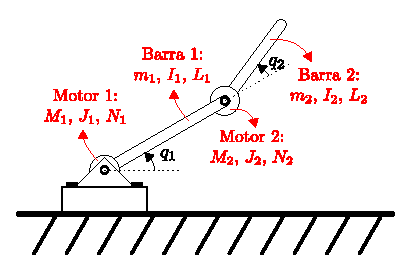
\includegraphics[width=0.5\linewidth]{figures/manipulador.eps}
\caption{Representação do sistema de servomotores com dois braços, no caso plano.}
\label{fig:manipulador}
\end{figure}

Um esquema do caso estudado para este relatório, o qual já corretamente representa a situação nas juntas de robôs humanoides, pode ser visto na figura \ref{fig:manipulador}. Nela, $M_i$, $J_i$, $N_i$, $m_1$, $I_i$ e $L_i$, referem-se, respectivamente, à massa do motor $i$, momento de inércia do motor $i$, razão de transferência do motor $i$, massa da barra $i$, momento de inércia da barra $i$ em relação ao eixo passando pelo seu centro de massa e comprimento da barra $i$, para $i = 1,2$. Considerando as barras homogêneas, adota-se a relação em .

\begin{equation}
\label{eq:inerciabarra}
I_i = \frac{m_i L_i^2}{12}.
\end{equation}

Inicialmente, observa-se que, para a modelagem, convém usar as equações de Euler-Lagrange, técnica comum na literatura de manipuladores \cite{craig1986}. Como marcado na figura \ref{fig:manipulador}, as coordenadas generalizadas adotadas serão os ângulos relativos a linha de base anterior, $q_1$ e $q_2$.

Tomando os momentos de inércia das barras nos eixos em seu centro de massa, faz-se necessário descrever a velocidade do centro de massa da barra $2$ (as velocidades dos demais elementos são imediatas), descrito em \ref{eq:vg2}, em que $\vec{v}_{G_2}$ é a velocidade do centro de massa da barra $2$, $V_{M_2}$ é a velocidade do motor $2$, $\vec{k}$ é o vetor unitário normal ao plano e $\vec{r_2}$ é o vetor unitário na direção da barra $2$. Com isso, é possível calcular a energia cinética de cada elemento por \eqref{eq:encinqqer}, em que $m^{CM}$ e $I^{CM}$ são, respectivamente, a massa e momento de inércia dos centros de massa de elementos quaisquer e $\omega$ e $v^{CM}$ são, em ordem, a velocidade angular e linear no centro de massa em relação ao solo. A energia cinética total a soma da energia cinética em cada elemento. 


\begin{equation}
\label{eq:vg2}
\vec{v}_{G_2} = \vec{v_{M_2}}+\frac{L_2}{2}(\dot{q_1}+\dot{q_2})(\vec{k} \times \vec{r_2}).
\end{equation}

\begin{equation}
\label{eq:encinqqer}
T_i = \frac{I^{CM} (\omega)^2}{2} + \frac{m^{CM} (v^{CM})^2}{2}.
\end{equation}

As energias cinética e potencial, representadas em \eqref{eq:cinetica} e \eqref{eq:potencial}, sendo $g$ a aceleração da gravidade, respectivamente, geram $L = T-V$. Das relações em\eqref{eq:lagrange}, ignorando atritos, obtém-se, por fim, as equações dinâmicas do conjunto de servomotores.

\begin{equation}
\begin{aligned}
\label{eq:cinetica}
T = \frac{J_1 N_1^2 \dot{q_1}^2}{2} &+ \frac{m_1}{2}\left(\frac{dot{q_1}L_1}{2}\right)^2+\frac{1}{2}\frac{m_1 L_1^2 \dot{q_1}^2}{12}+\frac{M_2 \dot{q_2}^2 L_1^2}{2}+\frac{J_2(N_2 \dot{q_2}+\dot{q_1})}{2}\\ &+\frac{m_2 \dot{q_1}^2 L_1^2}{2} + \frac{m_2 (\dot{q_1}+\dot{q_2})^2 L_2^2}{6} + \frac{m_2 \dot{q_1}(\dot{q_1}+\dot{q_2})}{2}L_1 L_2 \cos q_2.
\end{aligned}
\end{equation}
\begin{equation}
\label{eq:potencial}
V = m_1 g \frac{L_1}{2} \sin q_1 + M_2 g L_1 \sin q_1 + m_2 g \left[L_1 \sin q_1 + \frac{L_2}{2} \sin (q_1 + q_2)\right].
\end{equation}

\begin{equation}
\label{eq:lagrange}
\frac{d}{d t}\left(\frac{\partial L}{\partial \dot{q_i}} \right) - \frac{\partial L}{\partial q_i} = 0, i = 1,2.
\end{equation}

Finalmente, obtém-se as equações do sistema dinâmico, em função de $q = [q_1 q_2]^T$, desconsiderando atritos ou entradas de torque, em \eqref{eq:dinamica}. Na matriz $\mathcal{J}$, em \eqref{eq:J}, estão destacados os termos que motivam esta dedução, que introduzem inércia em primeira ordem em $N_2$. Na literatura, com algumas excessões encontradas pelos autores \cite{siciliano,nasareport}, costuma-se desprezar estes termos, frente aos termos quadráticos de $N_1$ e $N_2$. Para diversas aplicações, como a do controle de caminhada, pode haver influência considerável destes termos \cite{nasareport}, o que motiva este estudo. 

\begin{equation}
\label{eq:dinamica}
B(q) \ddot{q} + C(q, \dot{q}) \dot{q} + g(q) = 0,
\end{equation}
em que:
\begin{equation}
B(q) = \begin{bmatrix} \frac{m_1 L_1^2 + m_2 L_2^2}{3} + m_2 L_1^2 + m_2 L_1 L_2 \cos q_2 & \frac{m_2 L_2^2}{3}+\frac{m_2 L_1 L_2 \cos q_2}{2}\\ \frac{m_2 L_2^2}{3}+\frac{m_2 L_1 L_2 \cos q_2}{2} &\frac{m_2 L_2^2}{3} \end{bmatrix} + \mathcal{J},
\end{equation}
\begin{equation}
\label{eq:J}
\mathcal{J} = \begin{bmatrix} M_2 L_1^2 + J_2 + J_1 N_1^2 & \textcolor{red}{J_2 N_2} \\ \textcolor{red}{J_2 N_2} & J_2 N_2^2 \end{bmatrix},
\end{equation}
\begin{equation}
C(q,\dot{q})=m_2 L_1 L_2 \sin q_2 \begin{bmatrix} -\dot{q_2} & -1/2 \dot{q_2} \\ 1/2 \dot{q_1} & 0 \end{bmatrix},
\end{equation}
\begin{equation}
g(q) = g \begin{bmatrix} m_1 \frac{L_1}{2}\cos q_1 + m_2 \left(L_1 \cos q_1 + \frac{L_2}{2} \cos (q_1+q_2) \right) + M_2 L_1 \cos q_1 \\ m_2 \frac{L_2}{2} \cos (q_1+q_2) \end{bmatrix}.
\end{equation}
\subsection{Estensão do modelo para um robô humanoide}
Embora a dedução tenha sido feita para apenas dois membros, é possível estender o modelo para o robô como um todo. Utiliza-se esta modelagem para uma malha de controle em baixo nível com ganhos constantes, de modo que não se faz necessário resolver o problema a tempo de iteração.
\subsection{Compensador de orientação do torso}

Como mencionado, a malha de controle da caminhada costuma ser dividida em níveis. No presente projeto, o estudo da equação do manipulador será utilizado para o projeto de um compensador da orientação do torso, marcado em vermelho na figura \ref{FIG: doc manga}, adaptada de \cite{tesemarcos}, da malha de controle da caminhada. Trata-se de um controlador P-V, proporcional
\begin{figure} 
	\centering
	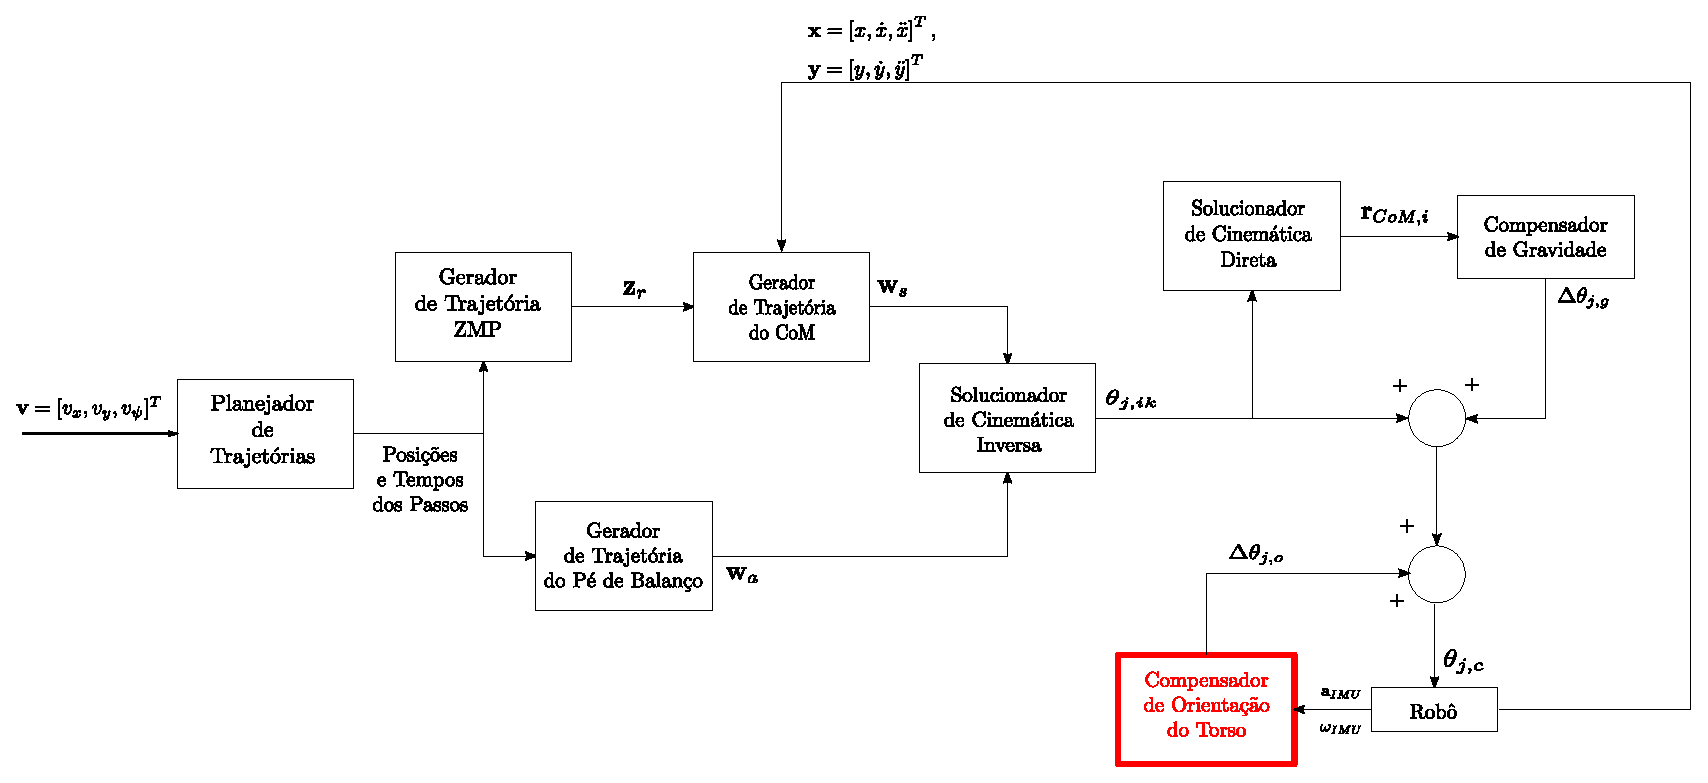
\includegraphics[angle=90, height = 0.9\vsize]{figures/walking_engine_overview.eps}
	\caption{Visão geral do controle de caminhada.}
	\label{FIG: doc manga}
\end{figure} 

A malha de controle do primeiro robô Chape, do LAB-SCA, levou em consideração correções feitas por testes, referente a falha na utilização do modelo de simulador Gazebo para a aplicação de redução nos motores, pois, como mencionado, este, por padrão, ignora o termo linear da razão de redução.

Assim, estuda-se esta modelagem como possível candidata a otimização da malha de controle atual e a sua completa aplicação no novo robô humanoide Chape, segunda geração. Uma correta aplicação no projeto simulado e na determinação dos ganhos do controlador deve proporcionar melhor resposta em algumas faixas do movimento.

\section{Algoritmos de otimização}

Com a malha de controle em baixo nível do compensador do torso, faz-se necessário otimizar os ganhos do controlador P+V utilizado. No projeto do robô Chape de segunda geração, será necessário reestudar os ganhos já projetados para o modelo anterior.

Para todas as etapas do controlador, em geral, realizam-se otimizações de modo a minimizar uma função custo do controlador. A função será escolhida segundo métodos já conhecidos, e minimizar a função custo costuma ser o objetivo da otimização. O problema é montado, de forma genérica, na relação \eqref{eq:min}, em que $g_i$ e $h_j$ são as restrições em desigualdade e igualdade que o sistema exige. Uma restrição, por exemplo, pode ser a faixa de atuação dos servomotores de um manipulador com barreiras físicas em seu movimento.

\begin{equation}
\label{eq:min}
\begin{aligned}
\underset{x}{\min} & J(x)\\
\text{sujeita a: } & g_i(x) \leq 0, i = 1, ..., m.\\
& h_j(x) = 0, j = 1,...,p. 
\end{aligned}
\end{equation}

Há diversos algoritmos de minimização de funções, podendo envolver ou não restrições. O escolhido para esta aplicação é o algoritmo simplex, ou Nelder-Mead, que funciona baseado em uma busca por mínimos com a variação de politopos em torno do estado em cada iteração de forma heurística \cite{NoceWrig06}.

\subsection{Uso do algoritmo simplex}

A função fminsearch utiliza o algoritmo simplex e se mostra adequado para a complexidade das malhas de controle na qual será utilizado. A única ressalva a ser feita é a sua sensibilidade ao ponto inicial $x_0$ passado. Costuma-se cair em mínimos locais da função custo, dado um $x_0$ muito longe do ótimo.

Uma estratégia a ser utilizada é a solução de modelos mais simples, que possam ser resolvidos de forma analítica. Havendo o $x^*$ ótimo para esse problema simplificado, pode-se adotar $x_0 = x^*$ como chute inicial.

Como já existe uma solução prévia para o problema, no robô Chape. A otimização de um código modificado neste robô ou a implementação do código para a segunda geração Chape já possui um chute inicial dos ganhos P+V utilizados atualmente.

\subsection{Aplicação em malha de corrente}

Para exercitar a aplicação, foi estudado o modelo de um servomotor de posição genérico \cite{max27} com malha de corrente. Para a malha de corrente, a ideia era implementar, por meio do método de projetos em frequência, um controlador do tipo Lead combinado em série com um integrador. Foi considerado além da planta o efeito de atraso da discretização e o controle, havendo retorno unitário.

Para isso, inicialmente foi resolvido o problema analítico da planta simplificada. Então, com o ponto original para a otmização, aplicou-se a função fminsearch na função de ganho $J(x)$ apresentada em \eqref{eq:ganhocorrente}, em que $K$ representa de forma genérica as constantes do controlador e $\omega_b^d$ e $PM^d$ são, respectivamente, a banda passante e a margem de fase desejados no projeto, enquanto $\omega_b(K)$ é a banda passante para $K$ atual na iteração  e $PM(K)$, a fase de margem.

\begin{equation}
\label{eq:ganhocorrente}
J_c(K) = (\omega_b^d - \omega_b(K))^2+(PM^d-PM(K))^2.
\end{equation}

A formulação desta função de custo na forma quadrática já foi suficiente para resolver o problema de otimização, indicando que a aplicação no projeto do compensador P+V pode ser feita de forma semelhante. Espera-se maior complexidade visto que o robô humanoide possui mais graus de liberdade, mas a ideia de projeto segue a mesma aplicação.

\section{Plano de trabalho e cronograma para as etapas seguintes}

Seguindo-se as etapas restantes, espera-se focar boa parte do trabalho no período de férias de graduação do aluno, período compreendido de dezembro de 2020 a março de 2021. 

Como mencionado, o principal objeto de estudo para otimização estão na malha em baixo nível, dos ganhos obtidos da otimização do controlador P+V do compensador de orientação do torso. O foco do estudo, portanto, será nesses aspectos, iniciando por um estudo a fundo do código atual do robô Chape, da implementação do controle e determinação dos ganhos.

Pretende-se seguir o cronograma e atividades a seguir, com pequenas modificações no foco quanto ao proposto inicialmente:

\begin{enumerate}[A]
\item{Estudo detalhado do código do robô humanoide relacionado ao seu caminhar e organização do código;}
\item{Continuação do processo de otimização;}
\item{Estudo do modelo implementado do compensador de orientação de torso;}
\item{Testes no robô real seguidos de aquisição de dados;}
\item{Fim do processo de otimização seguido da comparação de resultados do antes e pós processo de modificação e otimização;}
\item{Implementação definitiva do novo código;}
\item{Ajuste na malha de controle para melhor desempenho;}
\item{Confecção do segundo relatório científico.}
\end{enumerate}

\begin{table}[h!]
	\centering
	\caption{Cronograma de atividades futuras.}
	\label{tab:CronogramaFinal}
		\begin{tabular}{|c|C|C|C|C|C|C|C|C|}
		\hline
		\multirow{2}{*}{Mês} &  \multicolumn{8}{c|}{Atividade} \\
		 & \multicolumn{1}{c}{A} & \multicolumn{1}{c}{B} & \multicolumn{1}{c}{C} & \multicolumn{1}{c}{D} & \multicolumn{1}{c}{E} & \multicolumn{1}{c}{F} & \multicolumn{1}{c}{G} & \multicolumn{1}{c|}{H}\\
		  \cline{2-9}
			Dez. & \cellcolor{gray!50} & &  &  &  &	 &  & \\
			\cline{2-9}
			Jan. & \cellcolor{gray!50} & \cellcolor{gray!50} & \cellcolor{gray!50} & & &	&  & \\
			\cline{2-9}
			Fev. &  & \cellcolor{gray!50} & \cellcolor{gray!50} & \cellcolor{gray!50} & &	&  & \\
			\cline{2-9}
			Mar. &  &  &  & \cellcolor{gray!50} &  & &  & \\
			\cline{2-9}
			Abril &  &  &  &  & \cellcolor{gray!50} & \cellcolor{gray!50} & \cellcolor{gray!50} &  \\
			\cline{2-9}
			Maio &  &  &  &  &  & \cellcolor{gray!50} & \cellcolor{gray!50} & \cellcolor{gray!50} \\
			\cline{2-9}
			Junho &  &  &  &  &  &	& & \cellcolor{gray!50} \\
					
			\hline
	\end{tabular}
\end{table}


%\section{Referências}

\newpage
\printbibliography
\end{document}